%no borrar PREAMBULO
\documentclass[12pt]{article}

\usepackage[top=3.5 cm, bottom=2.5  cm, left=3 cm, right=3 cm]{geometry}
\usepackage{fancyhdr}
\pagestyle{fancy}

\usepackage[hidelinks]{hyperref} %esta opción saca las cajas de colores de los hiperlinks

\fancyfoot[C]{\thepage }  %numera las páginas

\usepackage[utf8]{inputenc}

\usepackage{amsmath,amsfonts,amssymb}
\usepackage{xcolor}
\usepackage{fancyvrb}
\newcommand\verbbf[1]{\textcolor[rgb]{0,0,1}}%comando para colorear el texto en verbatim

%\linespread{1} %por si queremos achicar el espacio entre lineas

\usepackage{tabularx,booktabs}
\usepackage{graphicx}
\usepackage{float} %para que las figuras puedan ponerse en cualquier lado

\usepackage{subcaption}
\usepackage{layout}
\usepackage{multicol}  %para escribir en columnnas 
\usepackage{float}
\usepackage{textcomp}
\usepackage{natbib}
\usepackage{tikz}
\usepackage{multirow} %para cambiar el alto de una fila en una tabla
\tikzset{
  connect/.style = { dashed, gray }
}
\usepackage{pgfplots}
\pgfplotsset{compat=1.8}
\usepackage[english ,spanish]{babel}
\usepackage{latexsym}
\usepackage{verbatim}

%\usepackage{alltt}
\usepackage{indentfirst}

\usepackage{fancybox, calc} 

\usepackage[flushmargin]{footmisc} %para alinear las notas de página

\usepackage{url}
\usepackage{advdate}
\usepackage{wrapfig}
\usepackage{amsthm}
\usepackage[inline]{enumitem} %para hacer listas en una linea, los mismos comandos con *
\newtheorem*{myteo}{Teorema} % la * es para no numerarlos
\newtheorem*{myexample}{Ejemplo}
\newtheorem*{myprop}{Proposición}
\newtheorem*{mylem}{Lema}
\theoremstyle{definition}
\newtheorem*{mydef}{Definición}
\newtheorem{ejer}{Ejercicio}
\newtheorem*{mydefs}{Definiciones}
%\theoremstyle{remark}
\newtheorem*{myobs}{Observación}
\newtheorem*{remark}{Importante}

\renewcommand{\baselinestretch}{1}  %interlineado

\addto\captionsspanish{%
  \renewcommand{\figurename}{Figura}%
}

\newcommand\myText[1]{\text{\scriptsize\tabular[t]{@{}l@{}}#1\endtabular}}
\addto\captionsspanish{%
  \renewcommand{\tablename}{Tabla}%
}

\def \ds {\displaystyle} %define un comando abreviado  
\def\com{“R”}

\usepackage{hyperref}%para referencias de internet con link!
\newcommand*{\fullref}[1]{\hyperref[{#1}]{ \nameref*{#1}}}
%comando \fullref para que ademas del número de capitulo, sección etc. escriba el título del capitulo, sección o lo que sea a lo que estamos haciendo referencia

\newcommand\comentario[1]{\textcolor{red}{#1}}%comentarios en el pdf

\interfootnotelinepenalty=10000 %previene que se pasen a otra página las notas de pie
\raggedbottom 
\addtolength{\topskip}{0pt plus 10pt}
\addtolength{\footnotesep}{0.1mm}

\VerbatimFootnotes%para poder usar Verbatim en las notas de pie

\begin{document}

\fancyhf{}
\pagestyle{fancy}
\lhead{Departamento de Matem\'{a}tica\\Universidad Nacional del Comahue}
\rhead{Matem\'{a}tica 1\\ Licenciatura en Ciencias Biol\'{o}gicas}

%HASTA ACA 

\begin{centering}
\Large{\textbf{Trabajo Práctico N° 1}}\\
\large{\textbf{Nociones básicas de conjuntos. Relaciones y operaciones}}\\
\end{centering}

\vspace{1cm}
\noindent
\textbf{Conjuntos: Nos ponemos de acuerdo con la notación.}\\
\noindent
Convencionalmente designaremos los conjuntos con letras mayúsculas y cuando queramos referirnos a alguno de sus elementos usaremos letras minúsculas. \\
La afirmación “el elemento $a$ \textbf{pertenece} al conjunto $A$” se escribe simbólicamente $a \in A$ y la negación de este hecho “el elemento $a$ \textbf{no pertenece} al conjunto $A$” se escribe $a \not \in A$.   \\
Las relaciones de inclusión que pueden darse entre conjuntos son: 
\begin{multicols}{4}
\noindent
\[ A \subset B \]
\[ B \supset A \]
\[ B \subseteq A \]
\[ B \supseteq A \]
\end{multicols}
En el primer caso decimos que  $A$ \textbf{está incluido} en $B$, en el segundo,  $B$ \textbf{incluye} a $A$. Los restantes admiten la posibilidad de que los conjuntos sean iguales.

\vspace{1cm}

\fbox{ \parbox{0.98\linewidth}{
\noindent
\textbf{IMPORTANTE}\\
\noindent
El símbolo (y el concepto) $ \in $ (o $ \not \in $) se refiere a una relación entre \textbf{un elemento} y \textbf{un conjunto}. 
El símbolo (y el concepto) $\subset$ (o $\not \subset$) se refiere a una relación entre \textbf{dos conjuntos}. 

}}

\vspace{1cm}
\noindent
Es decir, es incorrecto decir que un elemento \textbf{está incluido} en un conjunto. Un elemento \textbf{pertenece} o \textbf{no pertenece} a un conjunto. Los conjuntos se incluyen entre sí.\\

El símbolo $\varnothing$ denota el conjunto vacío. $ A = \varnothing$ indica que el conjunto $A$ no tiene elementos. La expresión $A = \{\varnothing \}$ es incorrecta, a menos que queramos indicar un conjunto que tiene ese símbolo como único elemento.\\
La definición de un conjunto no debe ser ambigua en el sentido de que debe poder decidirse cuándo un objeto particular pertenece o no al mismo.  Los conjuntos pueden estar definidos de diversas maneras. Diremos que están definidos \textbf{por extensión} cuando se especifican todos los elementos que forman el conjunto. Se dirá que están definidos  \textbf{por comprensión} cuando se indica la proposición que hacen cierta los elementos del conjunto. Un conjunto definido por comprensión tiene la forma: 
$ A = \{x \in R / x  \text{ verifica la proposición } p \} $, donde $R$ es un conjunto referencial.\\

Ejemplos:

\begin{enumerate} [leftmargin=2cm]%[a)]

\item Si nos referimos al conjunto formado por las vocales del alfabeto, su expresión por comprensión es, formalmente, $A = \{x \in R / x \text{ es una vocal}\}$, donde $R$ es el referencial constituido por las letras del alfabeto. Esta definición se lee “$A$ está formado por todos los elementos (que llamaremos genéricamente $x$) pertenecientes al referencial $R$, que verifican que $x$ es una vocal).\\
Por extensión: $A = \{a, e, i, o, u\}$.
\item El conjunto formado por los números enteros pares no negativos y menores que diez, se escribe:\\ Por comprensión como $B = \{x \in \mathbb{Z} / x \text{ es par, x es no negativo y } x < 10\}$.\\
Por extensión: $B = \{0, 2, 4, 6, 8\}$.\\
\end{enumerate}

\noindent
La ventaja de la definición por comprensión es que se explicita el conjunto referencial y la propiedad que deben verificar los elementos del conjunto, y que es adecuada aun para conjuntos donde la enumeración de los elementos es imposible (conjuntos infinitos).\\
\vspace{0.5cm}

\fbox{ \parbox{0.98\linewidth}{
\noindent
\textbf{Uso de las llaves.}\\
Las llaves se utilizan para encerrar la enumeración de los elementos de un conjunto, o para encerrar las proposiciones que verifican los elementos. Para nada más.  También para abrir puertas, pero esas son otras llaves.
}}


\begin{enumerate}
%1
\item Escribir los conjuntos siguientes por comprensión, explicitando claramente el referencial. Hacerlo lo más formalmente que puedas (no es obligatorio el uso de símbolos, sí la precisión):
\begin{multicols}{2}
$A = \{ 0, 1, -1, 2, -2, 3, -3 \}$ \\
$ B = \{ l, e, c, v, a \}$  \\
$C = \{ 1, 3, 5, 7, 9, 11, 13, 15, 17, 19 \}$\\
$D = \{1, 2, 3, 4, 6, 12 \}$   
\end{multicols}

%2
\item Escribir los siguientes conjuntos por extensión:\\
\begin{itemize*}
\item $A = \{x \in \mathbb{Z} /  5 < x \leq10\}$   ($\mathbb{Z}$ es el conjunto de los números enteros)\\	
\item $B = \{x \in \mathbb{N} /   \text{ x posee un dígito} \}$  \\
\item $C = \{x \in \mathbb{N} /   \text{ x es un divisor de } 10 \}$  \\
\item $D = \{x \in \mathbb{N} /   \text{ x es un número primo menor que 11} \}$  \\
\end{itemize*}

\noindent
Hemos visto las siguientes relaciones y operaciones entre conjuntos:

\begin{table}[ H]
\begin{center} 
\begin{tabular} { l l }
\textbf{Definición}& \textbf{Representación gráfica}\\ \hline  \\ 
%\hline
\begin{minipage}{10cm} El \textbf{complemento} de un conjunto $B$ es el conjunto que denotamos $ \overline B$ que contiene todos los elementos (respecto de algún conjunto referencial) que no pertenecen a $B$. \end{minipage} & \begin{minipage}{5cm} \begin{center} 
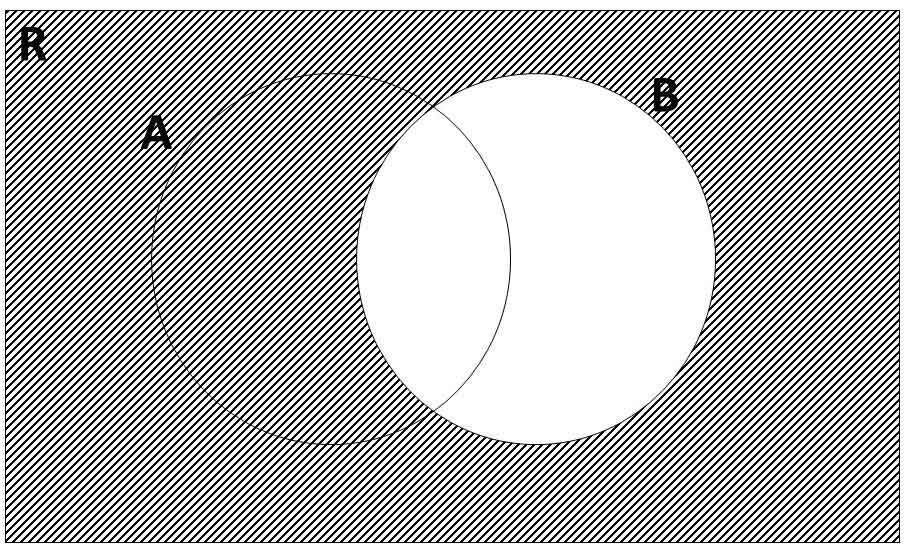
\includegraphics[width= 0.8\textwidth]{tp1_fig4.jpg} 
\end{center}
\end{minipage}\\ \\
\begin{minipage}{10cm} La \textbf{inclusión} de conjuntos $A \subset B$, es una relación que se verifica cuando todo elemento de $A$ es también elemento de $B$, aunque no necesariamente al revés. \end{minipage} & \begin{minipage}{5cm}  \begin{center} 
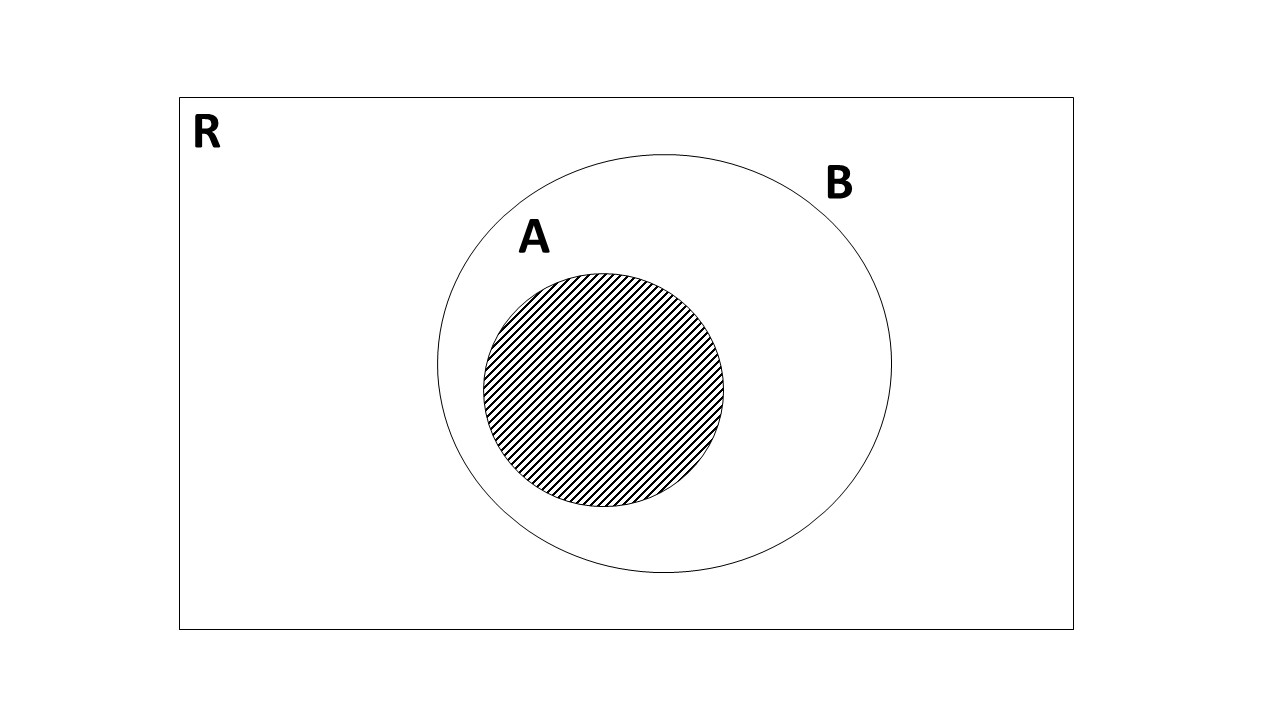
\includegraphics[width=0.8\textwidth]{tp1_fig1.jpg} 
\end{center}
\end{minipage}\\ \\   
\begin{minipage}{10cm} La \textbf{igualdad} de conjuntos $A = B$, indica que todo elemento de $A$ es también elemento de $B$ y viceversa.\end{minipage}& \begin{minipage}{5cm} \begin{center} 
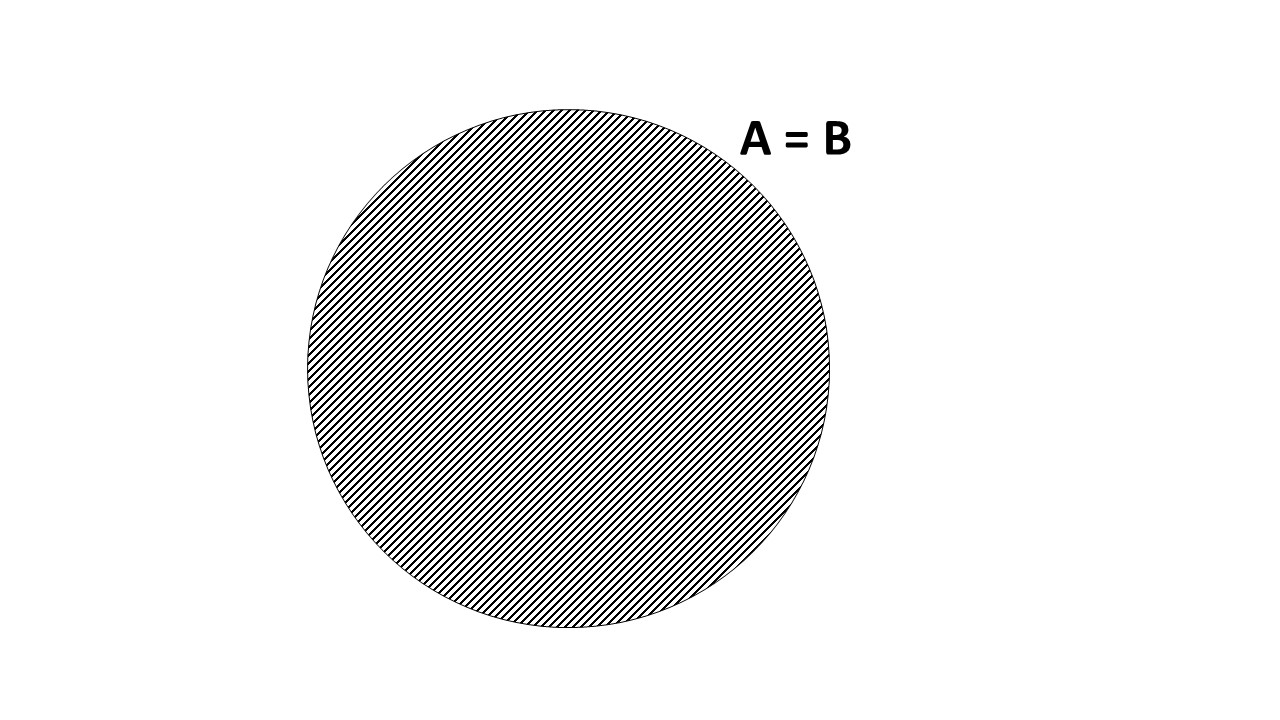
\includegraphics[width=0.8\textwidth]{tp1_fig9.jpg} 
\end{center}
\end{minipage}\\ \\ 
 \begin{minipage}{10cm} La \textbf{unión}, que denotamos $A \cup B$, representa un nuevo conjunto formado por los elementos comunes y no comunes de $A$ y de $B$. \end{minipage} &\begin{minipage}{5cm} \begin{center} 
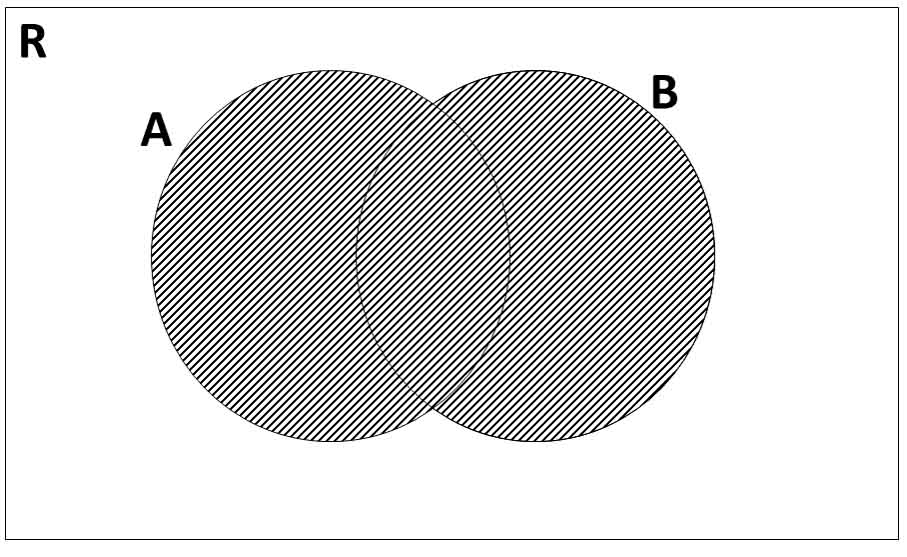
\includegraphics[width=0.8\textwidth]{tp1_fig5.jpg} 
\end{center}
\end{minipage}\\ \\  
\begin{minipage}{10cm} La \textbf{intersección}, que denotamos $A \cap B$, representa un nuevo conjunto formado por los elementos comunes de $A$ y de $B$. \end{minipage}& \begin{minipage}{5cm} \begin{center} 
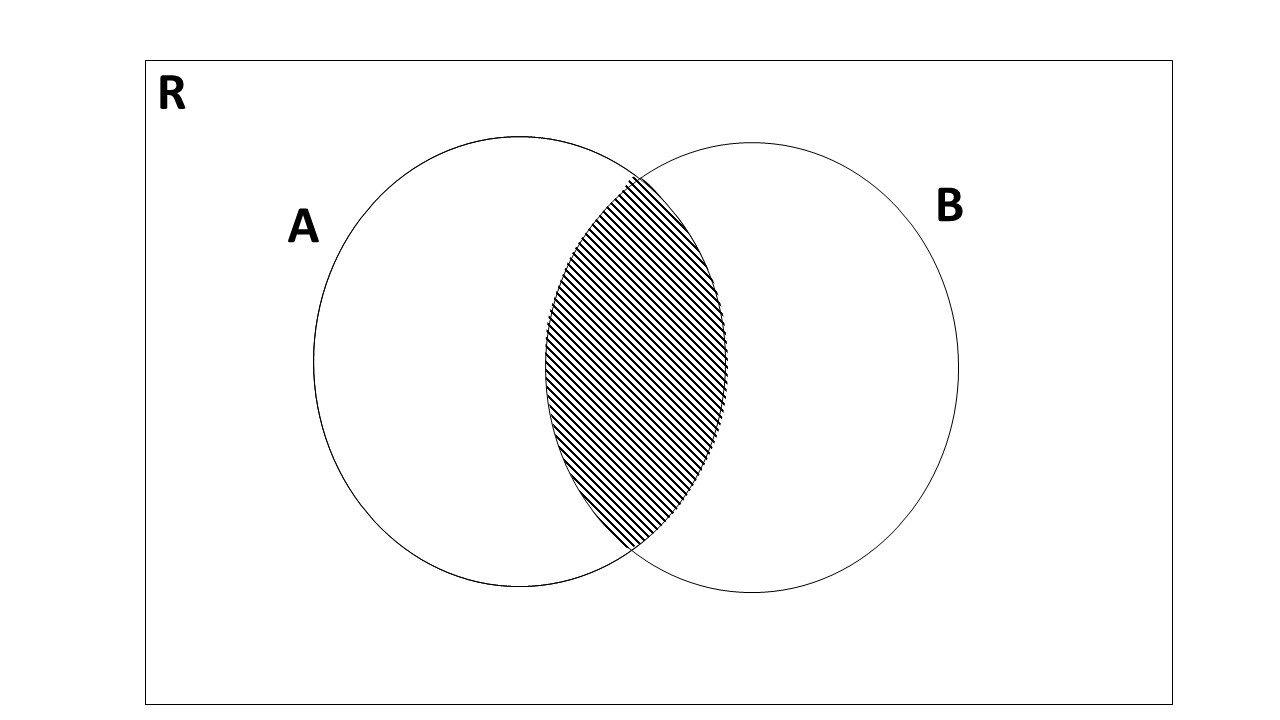
\includegraphics[width=0.8\textwidth]{tp1_fig10.jpg} 
\end{center}
\end{minipage}\\ \\  
\begin{minipage}{10cm} La \textbf{diferencia}, que denotamos $A -  B$, es el conjunto que contiene todos los elementos de $A$ que no pertenecen a $B$. \end{minipage} & \begin{minipage}{5cm} \begin{center} 
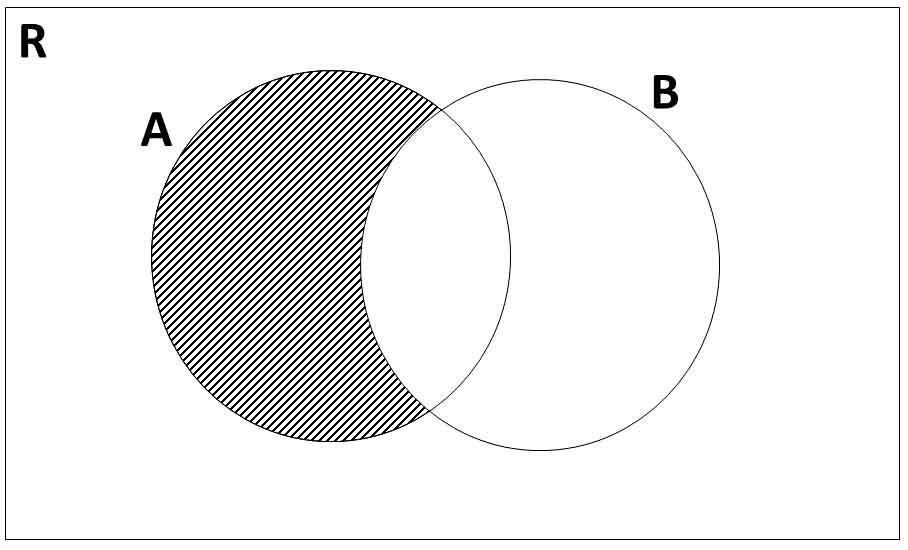
\includegraphics[width=0.8\textwidth]{tp1_fig7.jpg} 
\end{center}
\end{minipage}\\ \\ 
\begin{minipage}{10cm} La \textbf{diferencia simétrica}, que denotamos $A \Delta  B$, contiene todos los elementos que pertenecen, o bien a $A$, o bien a $B$, pero no a ambos a la vez. \end{minipage}& \begin{minipage}{5cm} \begin{center} 
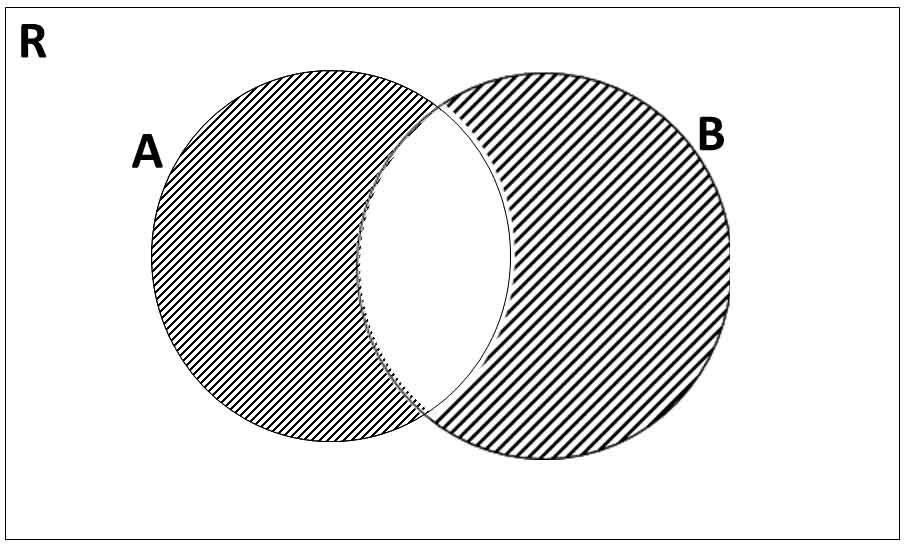
\includegraphics[width=0.8\textwidth]{tp1_fig8.jpg} 
\end{center}
\end{minipage}
\end{tabular} 
\end{center} 
\end{table}

%3
\item Dados los conjuntos $A = \{ 1 \}$ y $B = \{ 1,2 \}$, determinar si las siguientes afirmaciones están correcta o incorrectamente escritas. En cualquier caso explicar.  De las correctas, decir si son Verdaderas o Falsas y explicar.
\begin{table}[ H]
\begin{center} 
\begin{tabular} { c c c c c c c c c }
$A \subset B$ && $A \in B$ && $1 \subset B$ && $1 \in B$ && $B \subset A$ 
\end{tabular} 
\end{center} 
\end{table}

%4
\item Dados los siguientes conjuntos: $A= \{ 1,2,3,4 \}$, $B= \{ 2,4,6,8 \}$, $C = \{ 3,4,5,6 \}$  dentro del referencial $R = \{x \in \mathbb{N} /  x \leq 10 \}$ , hallar:
\begin{table}[ H]
\begin{center} 
\begin{tabular} { c c c c c c c c c }
 $A \cup B$ &&  $A \cup C$ &&  $B \cup B$ && $A \cap B$ && $A \cap C$ \\ \\
 $A \cap B \cap C$ &&  $A  - B $ &&  $C - A$ && $B - B$ && $ \overline A$ \\ \\
 $ \overline {A \cap B}$ &&  $ \overline {A \cup B}$ &&  $ \overline {A -B}$ && $ \overline {A \cup B \cup C}$ && $ \overline B$ \end{tabular} 
\end{center} 
\end{table}

%5
\item  Considerar los siguientes conjuntos de números naturales: \\
$U =  \{x \in \mathbb{N} / x  \text{ es menor que 10} \}$, \\
$A =  \{x \in \mathbb{N} / x  \text{ es un número primo y } x \leq 7 \}$\\
$B =  \{x \in \mathbb{N} / x  \text{ es un número par y }  x \leq 7 \}$\\

Determinar:
\begin{table}[ H]
\begin{center} 
\begin{tabular} { c c c c c c c c c c c c c c c }
 $\overline A$ &&  $\overline B$ &&  $A \cap \overline B$ && $\overline A \cup  \overline B$ && $B \cup \overline B$ &&
 $\overline B \cap A$ &&  $\overline B \cap U$ &&  $\overline {A \cup B}$ 
 \end{tabular} 
\end{center} 
\end{table}

%6
\item Escribir una operación entre los conjuntos $A$, $B$ y $C$ que dé por resultado la zona sombreada en las figuras siguientes:
 \begin{center} 
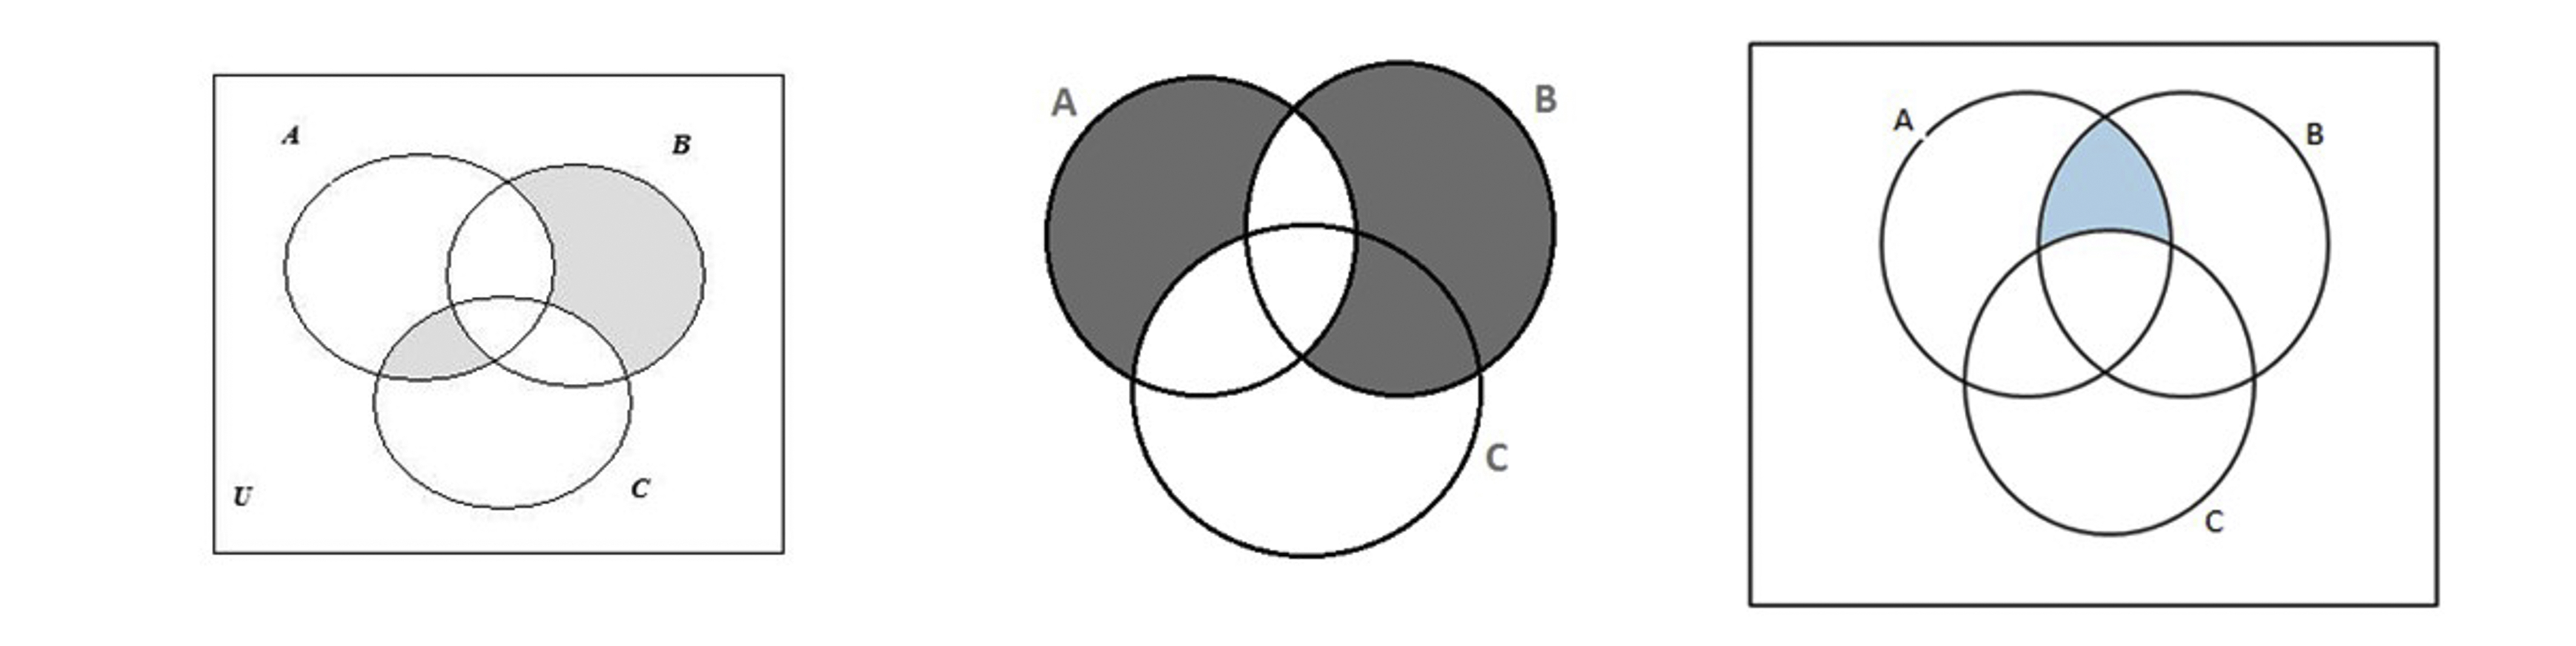
\includegraphics[width=1\textwidth]{tp1_fig11a.jpg} 
\end{center}
\begin{center} 
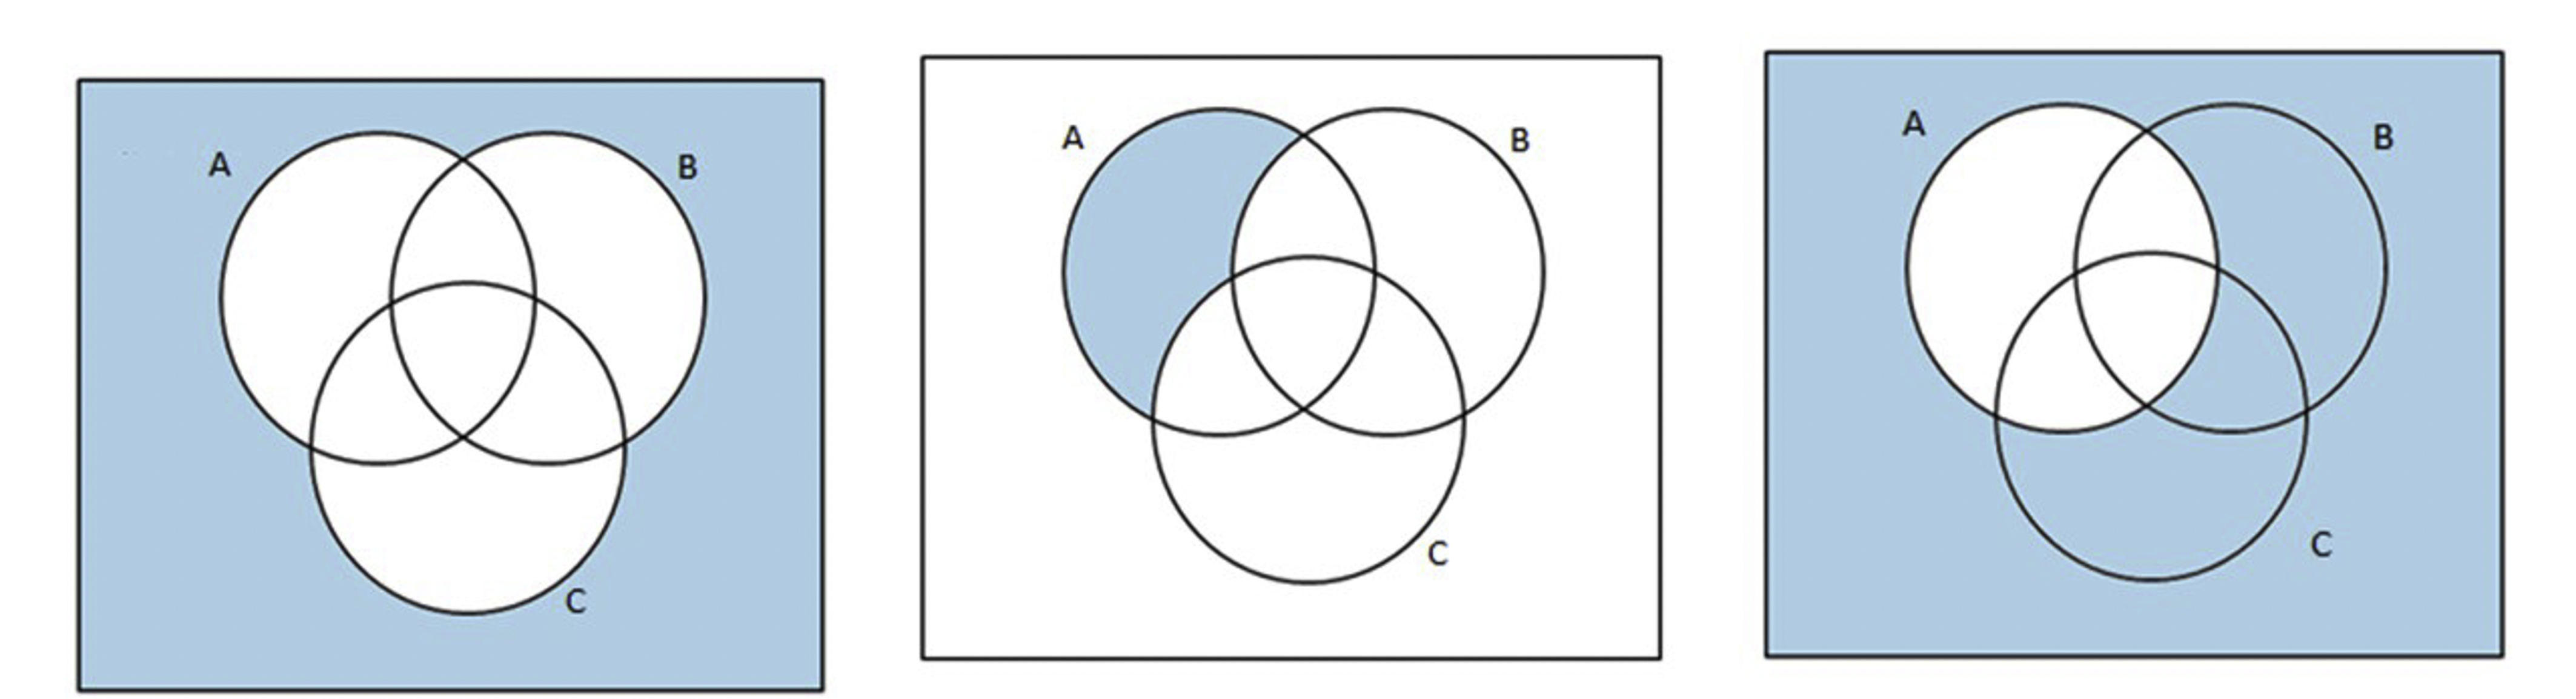
\includegraphics[width=1\textwidth]{tp1_fig11b.jpg} 
\end{center}

\textbf{Conjuntos desde el punto de vista de su cantidad de elementos} \\

%7
\item Distinguiremos tres categorías de conjuntos: el conjunto vacío (que representamos con el símbolo $\varnothing$), los conjuntos finitos y los conjuntos infinitos.  Decir de los siguientes conjuntos si son finitos, infinitos o vacíos:
\begin{enumerate}
\setlength\itemsep{0em}
\item Los números pares.
\item Los números enteros entre 0 y 10.
\item Los números reales entre 0 y 10.
\item Los átomos del universo.
\item Los pelos de las cabezas de todos los estudiantes de la Universidad del Comahue.
\item Los glóbulos rojos que tiene una persona en su torrente sanguíneo en un determinado día.
\item Los segundos transcurridos entre las 12 y las 13 hs
\item Los elefantes rosados.
\end{enumerate}

%8
\item Dar ejemplos de conjuntos finitos e infinitos.

%9
\item 	Escribir por extensión el conjunto $\{x \in \mathbb{Z} /  x \geq 0  \text{ y } x \leq 10\}$. ¿Cuántos elementos tiene?

%10
\item 	¿Cuántos elementos tiene el conjunto $\{x \in \mathbb{R} /  x \geq 0   \text{ y }  x \leq 10\}$? (no me equivoqué, no son iguales…).

%11
\item Proponer dos conjuntos finitos $A$ y $B$ tales que $A \cup B \neq \varnothing$ . ¿Qué se puede decir de la cantidad de elementos de la unión de $A$ y $B$? 
\end{enumerate}

\end{document}
